\documentclass{article} % say

\usepackage[utf8]{inputenc}
\usepackage{tikz}
\usetikzlibrary{mindmap,shadows}
\usepackage[hidelinks,pdfencoding=auto]{hyperref}

\newcommand*{\info}[4][16.3]{%
  \node [ annotation, #3, scale=0.65, text width = #1em,
          inner sep = 2mm ] at (#2) {%
  \list{$\bullet$}{\topsep=0pt\itemsep=0pt\parsep=0pt
    \parskip=0pt\labelwidth=8pt\leftmargin=8pt
    \itemindent=0pt\labelsep=2pt}%
    #4
  \endlist
  };
}

\begin{document}


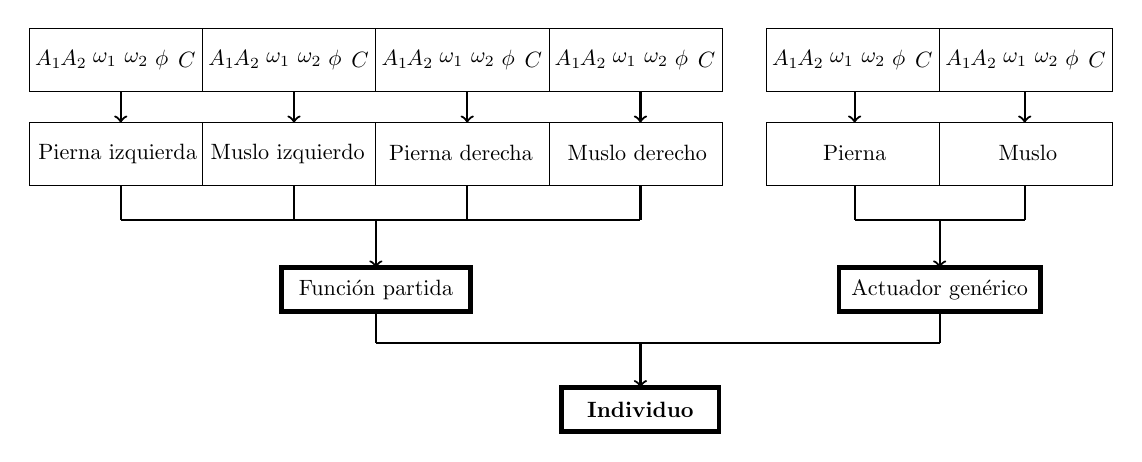
\begin{tikzpicture}[scale=0.8, every node/.style={scale=0.8}]
\def\rectanglepath[#1][#2]{-- ++(#1,0cm) -- ++(0cm,#2) -- ++(-#1,0cm) -- cycle}

\draw (6.7,-3.05) node[font=\bf, ultra thick]{Individuo};
\draw[thick,->] (6.7,-2) -- ++(0cm,-0.7cm) ;
\draw[ultra thick] (5.45,-3.4) \rectanglepath[2.5cm][0.7cm];
\draw[thick] (2.5,-2) -- ++(8.95cm,0cm) ;


\draw (2.5,-1.15) node{Funci\'on partida};
\draw[ultra thick] (1,-1.5) \rectanglepath[3cm][0.7cm];
\draw[thick] (2.5,-1.5) -- ++(0cm,-0.5cm) ;
\draw[thick,<-] (2.5,-0.8) -- ++(0cm,0.75cm) ;
\draw[thick] (-1.55,-0.05) -- ++(8.25cm,0cm) ;


\draw (11.45,-1.15) node{Actuador gen\'erico};
\draw[ultra thick]  (9.85,-1.5) \rectanglepath[3.2cm][0.7cm];
\draw[thick] (11.45,-1.5) -- ++(0cm,-0.5cm) ;
\draw[thick,<-] (11.45,-0.8) -- ++(0cm,0.75cm) ;
\draw[thick] (10.1,-0.05) -- ++(2.7cm,0cm) ;


\draw (-3,0.5) \rectanglepath[2.75cm][1cm];
\draw (-1.6,1) node{Pierna izquierda};
\draw[thick] (-1.55,0.5) -- ++(0cm,-0.55cm) ;

\draw (-3,2) \rectanglepath[2.75cm][1cm];
\draw (-2.7,2.5) node{$A_1$};
\draw (-2.3,2.5) node{$A_2$};
\draw (-1.8,2.5) node{$\omega_{1}$};
\draw (-1.3,2.5) node{$\omega_{2}$};
\draw (-0.9,2.5) node{$\phi$};
\draw (-0.5,2.5) node{$C$};
\draw[thick,->] (-1.55,2) -- ++(0cm,-0.5cm) ;


\draw (-0.25,0.5) \rectanglepath[2.75cm][1cm];
\draw (1.1,1.0) node{Muslo izquierdo};
\draw[thick] (1.2,0.5) -- ++(0cm,-0.55cm) ;


\draw (-0.25,2) \rectanglepath[2.75cm][1cm];
\draw (0.05,2.5) node{$A_1$};
\draw (0.45,2.5) node{$A_2$};
\draw (0.95,2.5) node{$\omega_{1}$};
\draw (1.45,2.5) node{$\omega_{2}$};
\draw (1.85,2.5) node{$\phi$};
\draw (2.25,2.5) node{$C$};
\draw[thick,->] (1.2,2) -- ++(0cm,-0.5cm) ;


\draw (2.5,0.5) \rectanglepath[2.75cm][1cm];
\draw (3.85,1.03) node{Pierna derecha};
\draw[thick] (3.95,0.5) -- ++(0cm,-0.55cm) ;

\draw (2.5,2) \rectanglepath[2.75cm][1cm];
\draw (2.8,2.5) node{$A_1$};
\draw (3.2,2.5) node{$A_2$};
\draw (3.7,2.5) node{$\omega_{1}$};
\draw (4.2,2.5) node{$\omega_{2}$};
\draw (4.6,2.5) node{$\phi$};
\draw (5.0,2.5) node{$C$};
\draw[thick,->] (3.95,2) -- ++(0cm,-0.5cm) ;


\draw (5.25,0.5) \rectanglepath[2.75cm][1cm];
\draw (6.65,1.03) node{Muslo derecho};
\draw[thick] (6.7,0.5) -- ++(0cm,-0.55cm) ;

\draw (5.25,2) \rectanglepath[2.75cm][1cm];
\draw (5.55,2.5) node{$A_1$};
\draw (5.95,2.5) node{$A_2$};
\draw (6.45,2.5) node{$\omega_{1}$};
\draw (6.95,2.5) node{$\omega_{2}$};
\draw (7.35,2.5) node{$\phi$};
\draw (7.75,2.5) node{$C$};
\draw[thick,->] (6.7,2) -- ++(0cm,-0.5cm) ;


\draw (8.7,0.5) \rectanglepath[2.75cm][1cm];
\draw (10.1,1.02) node{Pierna};
\draw[thick] (10.1,0.5) -- ++(0cm,-0.55cm) ;

\draw (8.7,2) \rectanglepath[2.75cm][1cm];
\draw (9.0,2.5) node{$A_1$};
\draw (9.4,2.5) node{$A_2$};
\draw (9.9,2.5) node{$\omega_{1}$};
\draw (10.4,2.5) node{$\omega_{2}$};
\draw (10.8,2.5) node{$\phi$};
\draw (11.2,2.5) node{$C$};
\draw[thick,->] (10.1,2) -- ++(0cm,-0.5cm) ;


\draw (11.45,0.5) \rectanglepath[2.75cm][1cm];
\draw (12.85,1.02) node{Muslo};
\draw[thick] (12.8,0.5) -- ++(0cm,-0.55cm) ;

\draw (11.45,2) \rectanglepath[2.75cm][1cm];
\draw (11.75,2.5) node{$A_1$};
\draw (12.15,2.5) node{$A_2$};
\draw (12.65,2.5) node{$\omega_{1}$};
\draw (13.15,2.5) node{$\omega_{2}$};
\draw (13.55,2.5) node{$\phi$};
\draw (13.95,2.5) node{$C$};
\draw[thick,->] (12.8,2) -- ++(0cm,-0.5cm) ;

\end{tikzpicture}

\newpage



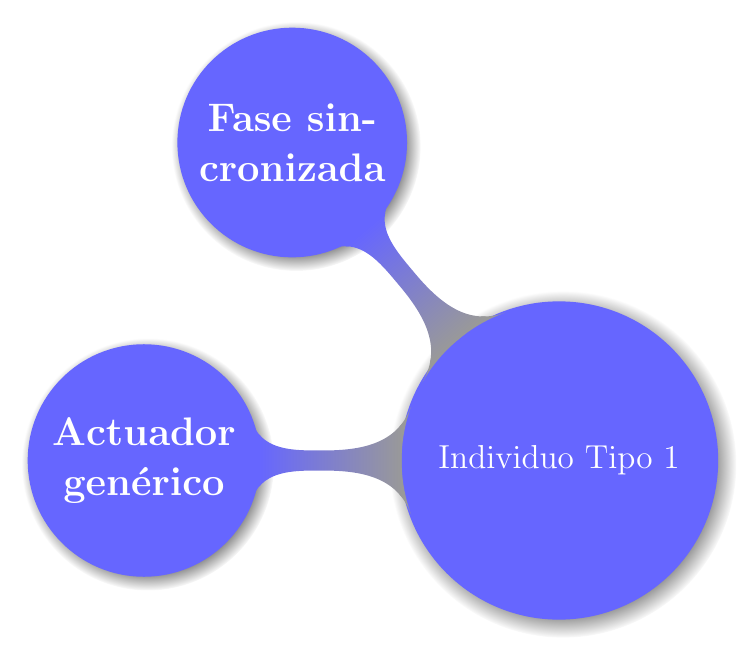
\begin{tikzpicture}[ every annotation/.style = {draw,
                     fill = white, font = \Large}]
  \path[mindmap,concept color=black!40,text=white,
    every node/.style={concept,circular drop shadow},
    root/.style    = {concept color=black!40,
      font=\large\bfseries,text width=10em},
    level 1 concept/.append style={font=\Large\bfseries,
      sibling angle=50,text width=7.7em,
    level distance=15em,inner sep=0pt},
    level 2 concept/.append style={font=\bfseries,level distance=9em},
  ]
  node[concept color=blue!60] {Individuo Tipo 1} [clockwise from=180]
    child[concept color=blue!60] {
      node {Actuador gen\'erico} [clockwise from=0]
    }
    child[concept color=blue!60] {
      node {Fase sincronizada} [clockwise from=90]
    }
    ;
   
\end{tikzpicture}



\end{document}